\section{Конструкторский раздел}
В данном разделе представлены диаграмма вариантов использования, диаграмма "сущность-связь"\ базы данных для хранения характеристик пользователя и IDEF0-диаграмма прикладной задачи определения усталости оператора АРМ.

\subsection{Диаграмма вариантов использования}
На рисунке \ref{fig:useCase} предоставлена диаграмма вариантов использования.
\begin{figure}[H]
	\centering
	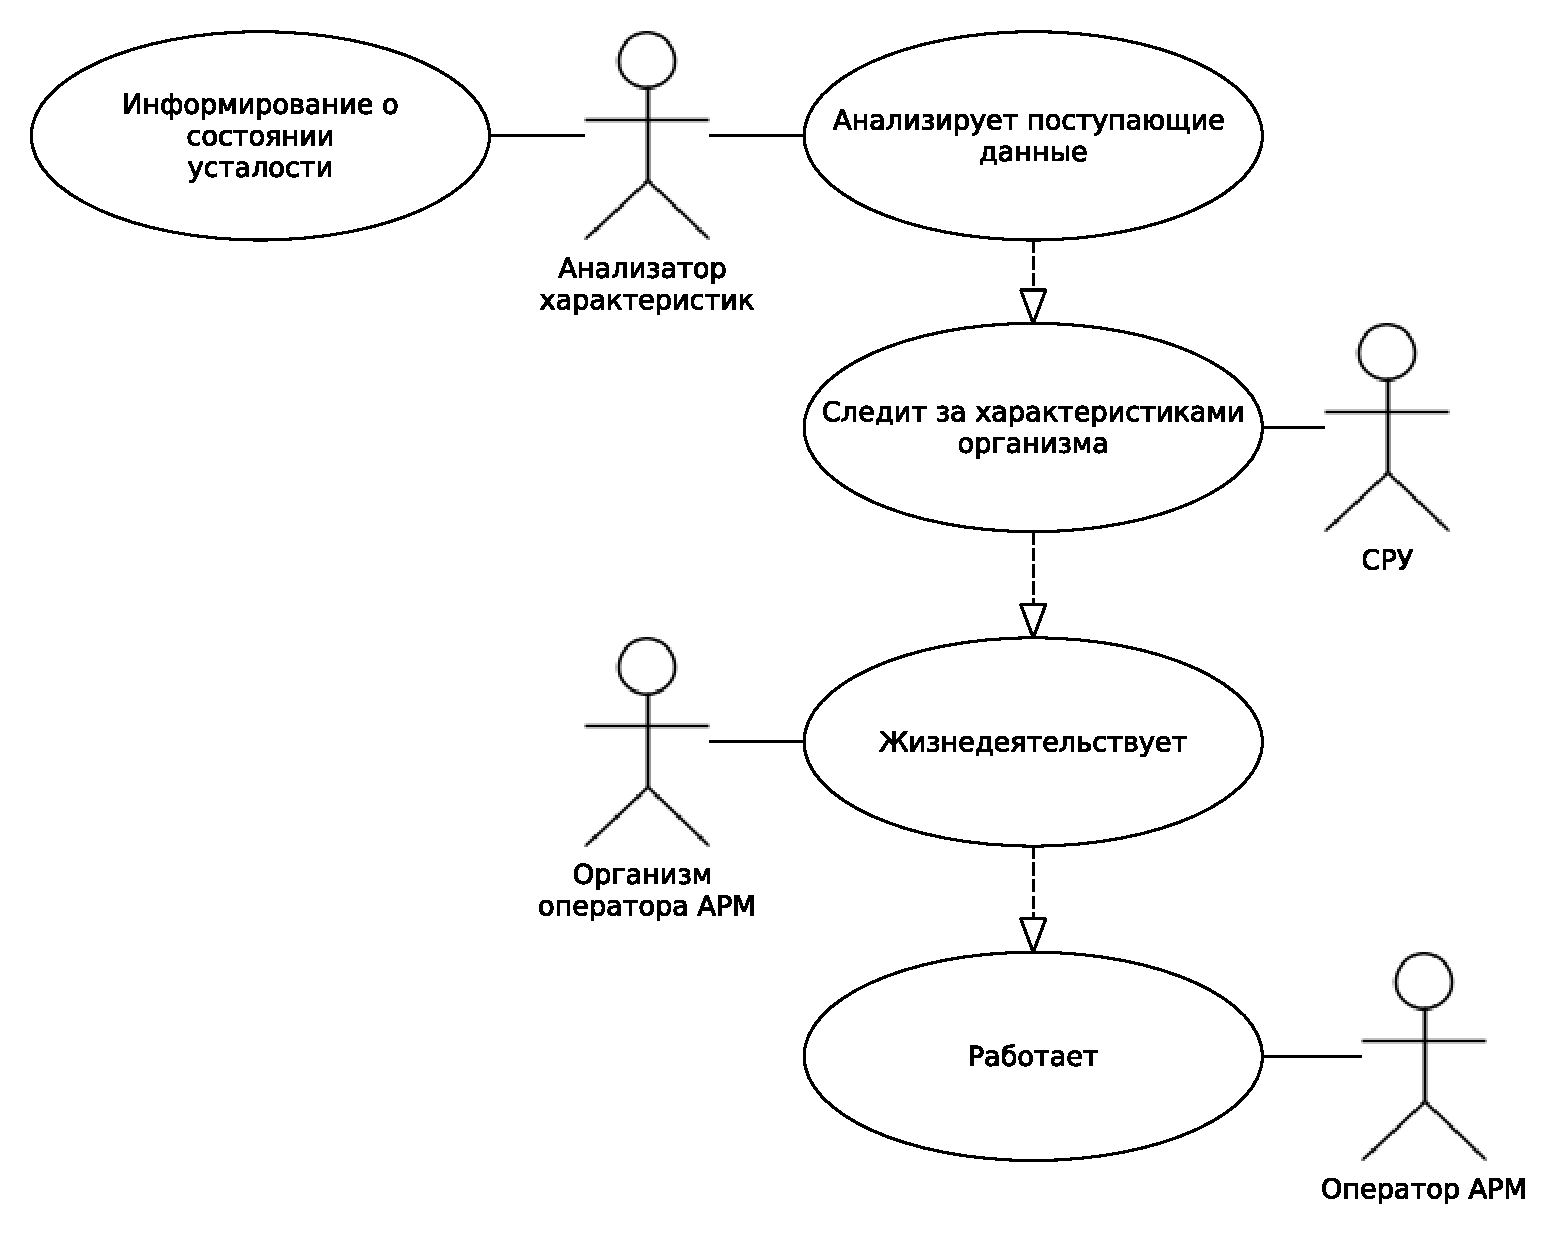
\includegraphics[width=\textwidth]{img/useCaseDiagramPresentation.pdf}
	\caption{Диаграмма вариантов использования.}
	\label{fig:useCase}
\end{figure}


\subsection{Диаграмма "сущность-связь"\ }
На рисунке \ref{fig:chen} предоставлена диаграмма "сущность-связь"\ базы данных для хранения характеристик пользователя в нотации Чена.
\begin{figure}[H]
	\centering
	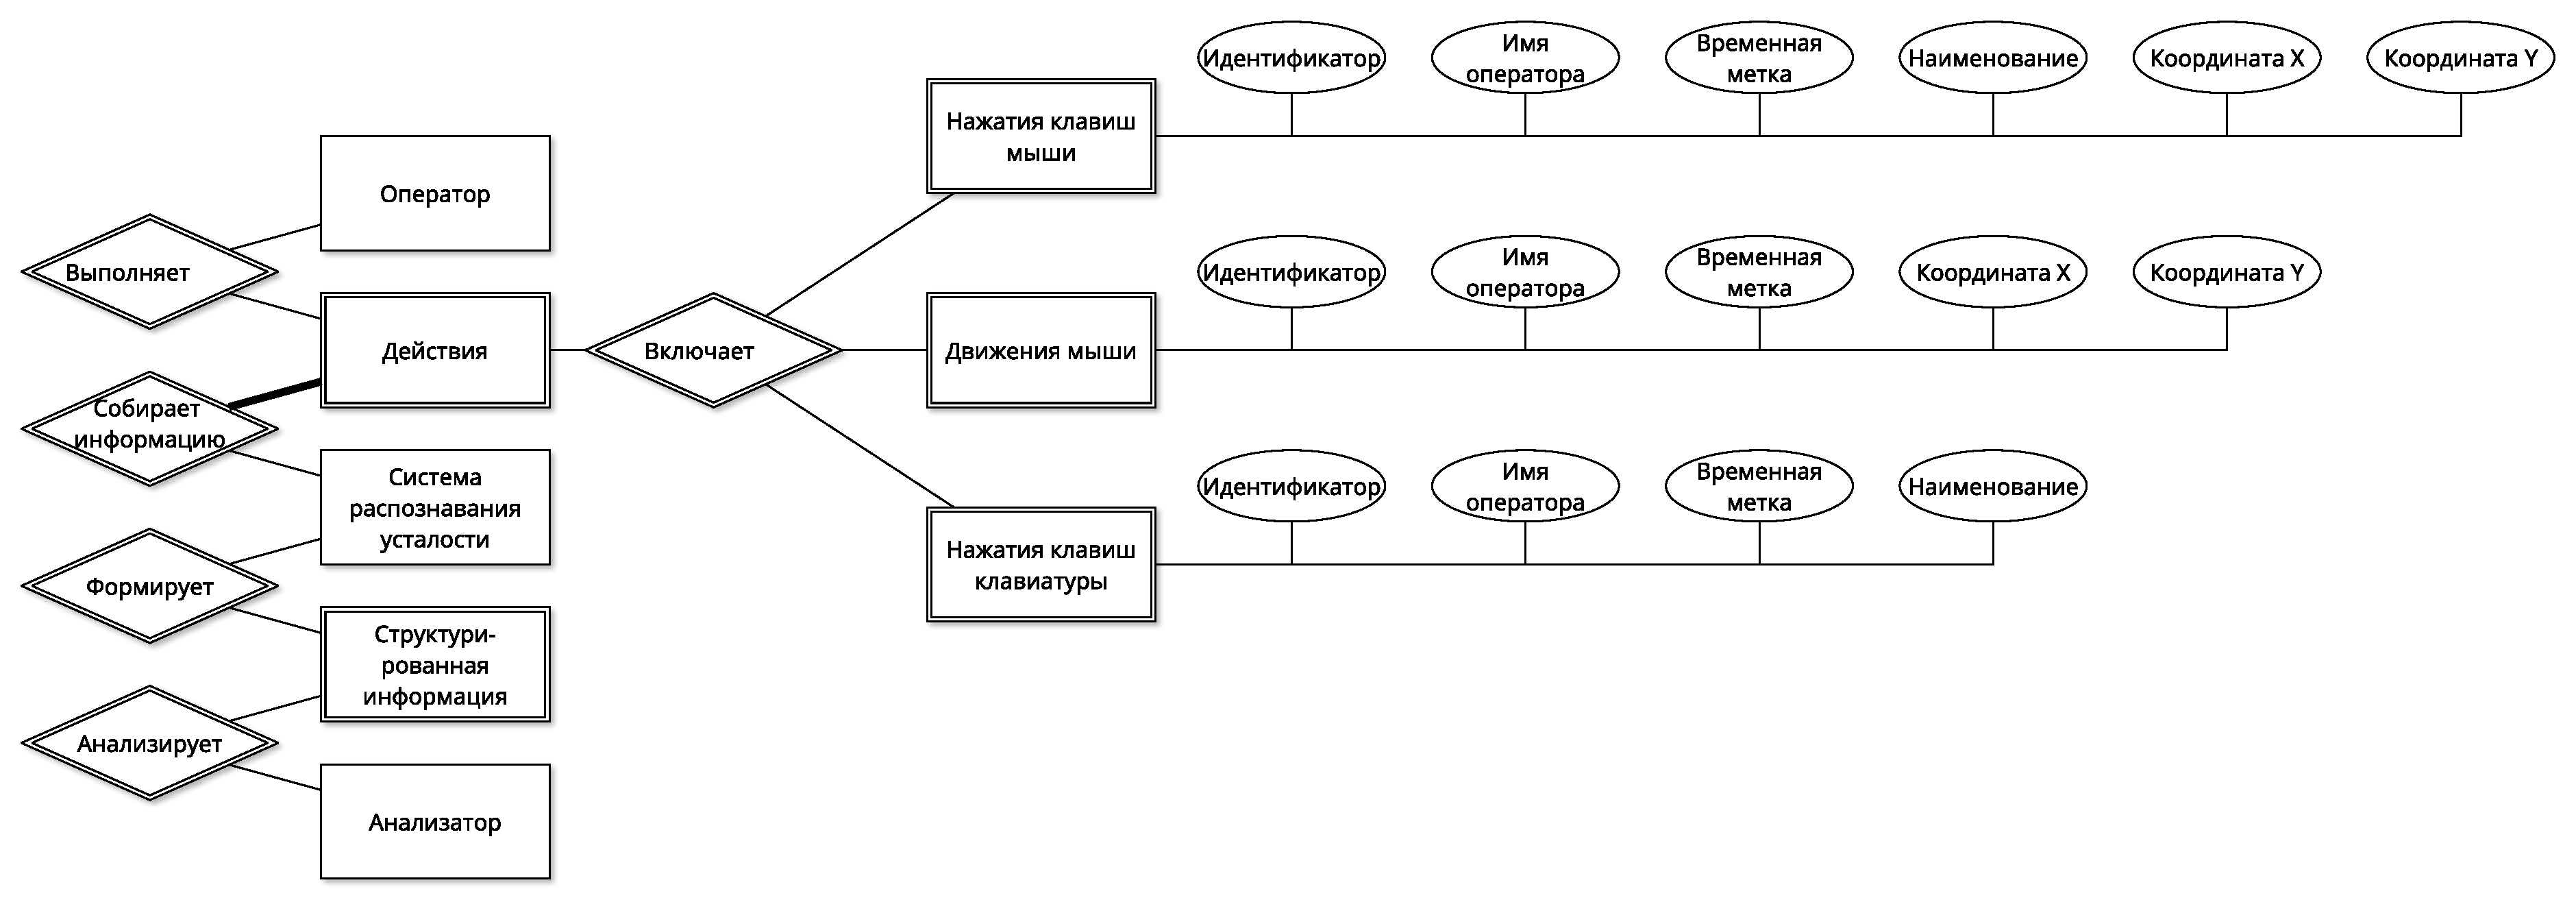
\includegraphics[width=\textwidth]{img/chenERDiagram.pdf}
	\caption{Диаграмма "сущность-связь"\ базы данных в нотации Чена.}
	\label{fig:chen}
\end{figure}

\subsection{IDEF0-диаграмма прикладной задачи}
На рисунках \ref{fig:idef:0}--\ref{fig:idef:1} предоставлена диаграмма IDEF0 прикладной задачи определения усталости оператора АРМ.

\begin{figure}[H]
	\centering
	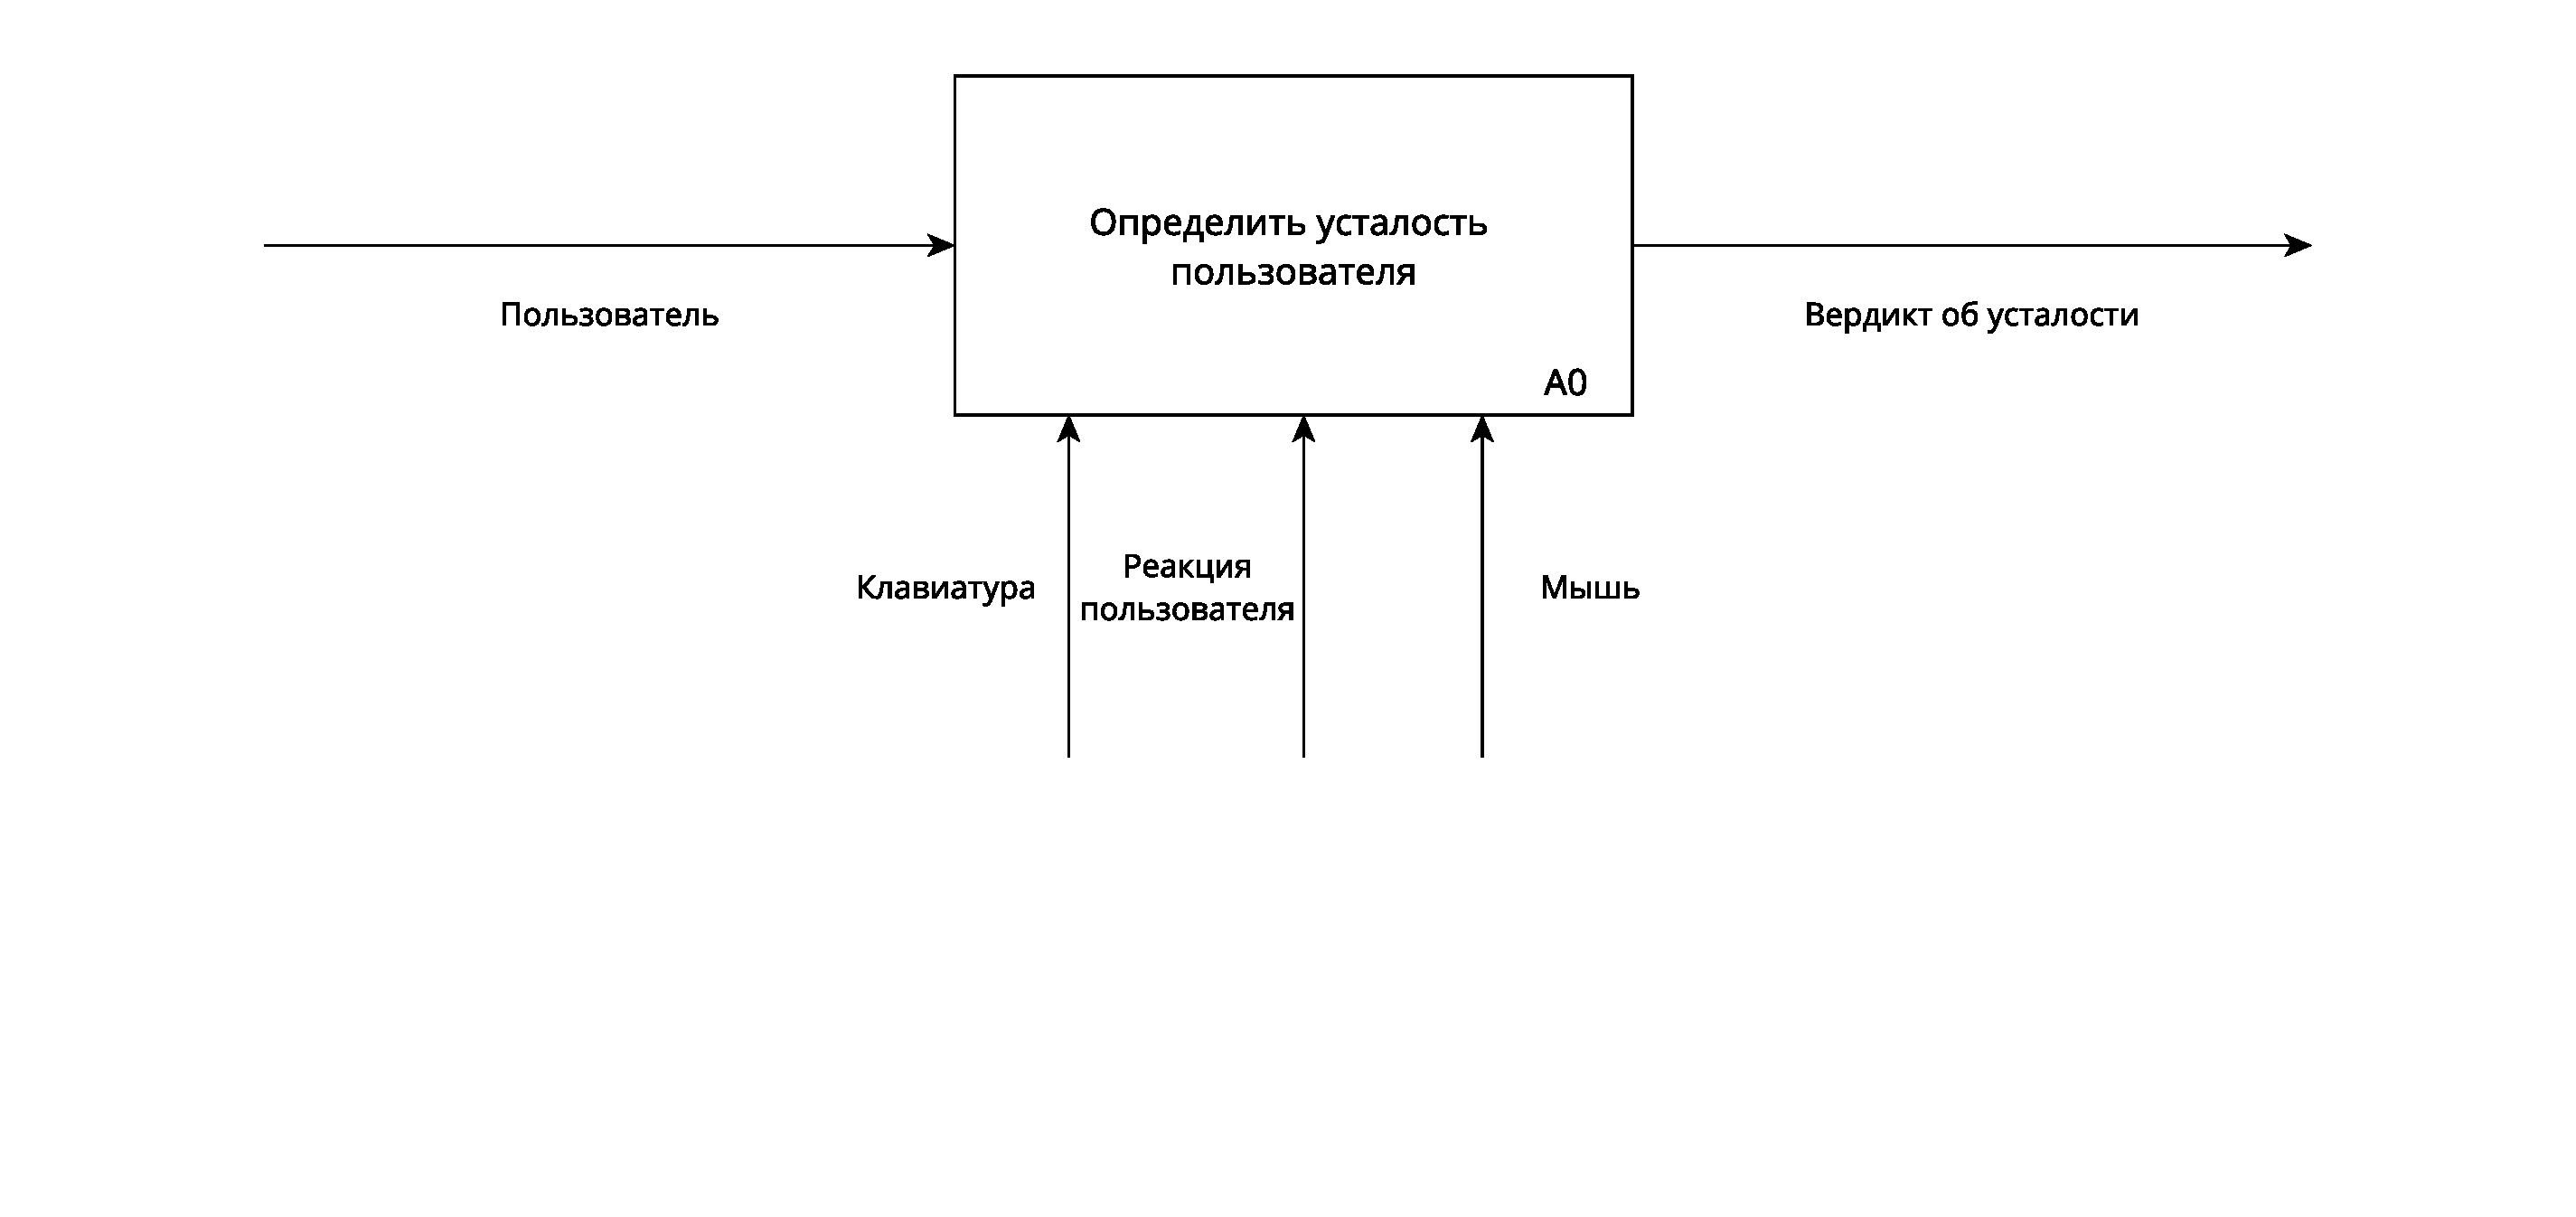
\includegraphics[width=\textwidth]{img/A0.pdf}
	\caption{IDEF0-диаграмма уровня A0.}
	\label{fig:idef:0}
\end{figure}

\begin{figure}[H]
	\centering
	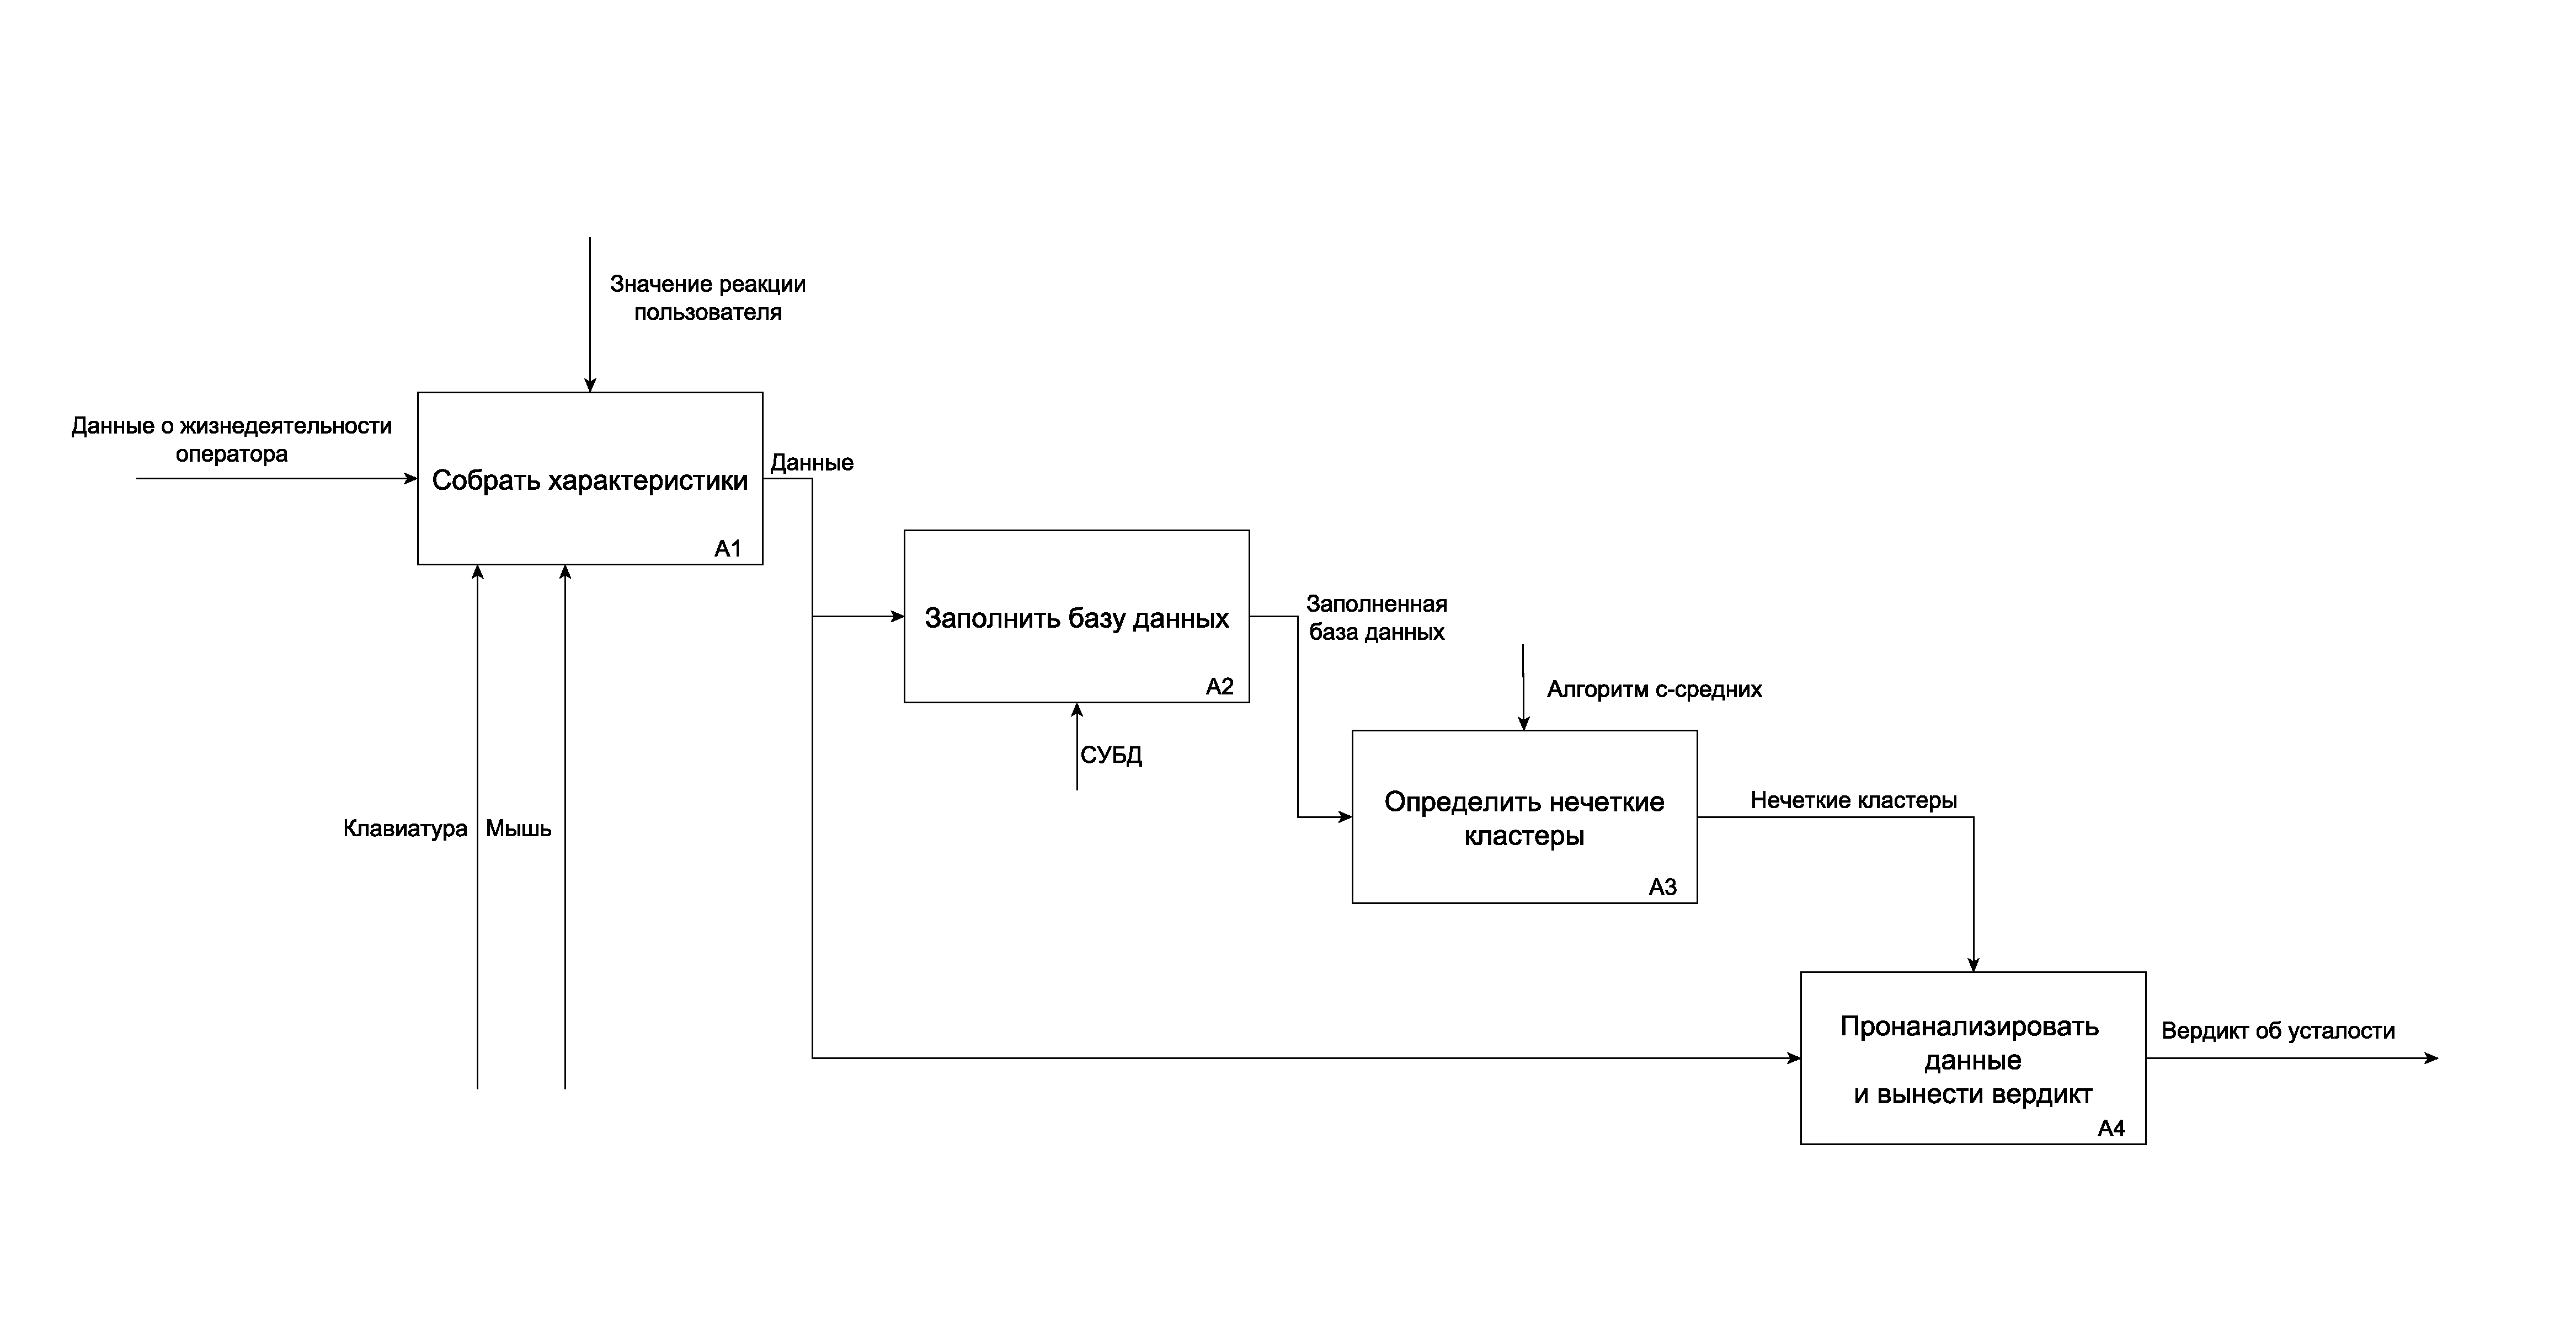
\includegraphics[scale=0.3]{img/A123.pdf}
	\caption{IDEF0-диаграмма уровня A1-A3.}
	\label{fig:idef:1}
\end{figure}

\subsection*{Вывод}
В разделе были представлены диаграмма вариантов использования, ER-диаграмма базы данных для хранения характеристик пользователя и IDEF0-диаграмма прикладной задачи.

Диаграмма вариантов использования позволила выделить 4 роли в системе: СРУ, анализатор характеристик, оператор АРМ, организм оператора АРМ.

Диаграмма "сущность-связь"\ включила в себя перечень выделенных характеристик из аналитического раздела и позволила описать базу данных для их хранения.

IDEF0-диаграмма позволила декомпозировать решаемую прикладную задачу.

\pagebreak